\documentclass[11pt]{article}
\usepackage [french]{babel}
\usepackage [T1]{fontenc}

\usepackage[linesnumbered, ruled, french, onelanguage]{algorithm2e}
\usepackage{adjustbox}%Permet de centrer les figures dans la largeur de la page même si les figures sont plus larges que \textwidth
\usepackage{amssymb}
\usepackage{amsmath}
\usepackage{adjustbox} % pour avoir adjustbox
\usepackage[toc,page,title,titletoc,header]{appendix}
\usepackage{expl3}%Pour la control sequence /ExlpSyntaxOn demandée par l'utilisation de subfiles apparemment...
\usepackage{gensymb}%pour pouvoir écrire le signe °
\usepackage{geometry}%Pour changer la largeur des marges du document notamment
\usepackage{graphicx}
\usepackage{hyperref}%pour les liens dans la bibliographie
\usepackage{listings}
\usepackage{placeins}%pour utiliser FloatBarrier afin que les figure respectent bien leur position dans le code
\usepackage{slashbox}%Case séparée en deux tout en haut à gauche des tableaux à double entrées
\usepackage{stmaryrd}%pour les crochets à double barres d'intervalles de nombre entiers
\usepackage{tikz}
\usepackage{xcolor}%/definecolor et /color
\usepackage{subfiles}

\usepackage{etoolbox}%pour /AtBeginEnvironment
\AtBeginEnvironment{appendices}{\renewcommand{\thesection}{\Alph {section}}}%Pour recommencer à compter les sections à 0 en rentrant dans l'annexe et pour compter avec des lettres et non des chiffres
\renewcommand{\appendixpagename}{\centering Annexes}%Pour centrer le titre de la partie annexe
\renewcommand{\appendixtocname}{Table des annexes} % Pour faire apparaître les annexes dans la table of contents
\setlength{\parskip}{2mm}%Pour mettre de l'espacement entre les paragraphes

%%%%%%%%%%%%%% Couleurs de: https://texblog.org/2011/06/11/latex-syntax-highlighting-examples/ %%%%%%%%%%%%%%
\definecolor{javared}{rgb}{0.6,0,0} % for strings
\definecolor{javagreen}{rgb}{0.25,0.5,0.35} % comments
\definecolor{javapurple}{rgb}{0.5,0,0.35} % keywords
\definecolor{javadocblue}{rgb}{0.25,0.35,0.75} % javadoc

\lstset
{
language=Java,
keywordstyle=\color{javapurple}\bfseries,
stringstyle=\color{javared},
commentstyle=\color{javagreen},
morecomment=[s][\color{javadocblue}]{/**}{*/},
numbers=left,
numberstyle=\tiny\color{black},
stepnumber=1,
numbersep=10pt,
tabsize=4,
showspaces=false,
showstringspaces=false}
%%%%%%%%%%%%%% Couleurs de: https://texblog.org/2011/06/11/latex-syntax-highlighting-examples/ %%%%%%%%%%%%%%





\author{Baptiste CLOCHARD \\
    Tom CLABAULT\\
    Thibaut LETOURNEUR\\
    Willie TANZIL}
\title{Ray-Tracer}
\date{}
\geometry{hmargin=3cm, vmargin=2cm}

\begin{document}
\maketitle
\newpage
\tableofcontents
\newpage

\maketitle

\section{Introduction}

    \subsection{Présentation du sujet}
        Le sujet que nous avons choisi pour ce projet est "Rendu 3D par lancer de rayon".
Le lancer de rayon (raytracing en anglais) est la simulation du comportement des rayons de lumière visant à créer des images 3D réalistes.
Ce sujet nous demandait d'implémenter :
\begin{itemize}
    \item Le parsing d'un fichier .pov
    \item La réflexion
    \item La réfraction
    \item L'ombrage de Phong
\end{itemize}
Nous avons réussi à implémenter tout ce qui était demandé pour le sujet.

    \subsection{Forme finale du projet}
        Tout en respectant le sujet, nous avons décidé d'implémenter un certain nombre de fonctionnalités facultative, mais qui nous semblait intéréssante.

Nous avons donc réalisé, en plus de ce qui était exigé par le sujet :
\begin{itemize}
    \item La gestion du rendu sur plusieurs threads.
    \item Le déplacement dans la scène 3d à l'aide de touches du clavier (avec actualisation de l'affichage en conséquence).
    \item le choix de la taille du rendu ainsi que son étirement possible pour conserver de la fluidité (mode automatique)
    \item L'usage d'une skybox.
    \item Les objets 3d possédant de la rugausité (raughness).
    \item L'ouverture et l'enregistrement du rendu 3D à l'aide de l'interface graphique.
    \item Le changement des parametres du rendu à la vollée (avec actualisation du rendu en conséquence).
    \item Un mode automatique permettant l'étirement propre de la fenêtre de rendu.
    \item L'ajout d'une texture en damier générée mathématiquement.
\end{itemize}

    \subsection{Répartition du travail}
        Assez tôt dans le projet le travail a été réparti et est resté pratiquement inchangé. Au final, voici les contributions de chacun :
\begin{description}
    \item [Tom] s'est chargé des structures mathématiques, des matériaux, des calculs du raytracing et de la gestion des threads
    \item [Baptiste] s'est occupé des réfractions, de la gestion et de l'affichage du rendu, du déplacement de la caméra et des possibilités offertes par l'interface graphique.
    \item [Thibaut] a codé le parser de fichier pov à l'aide d'un automate ainsi que les scripts de "déploiement".
    \item [Willie] a réalisé les différents objets 3D (formes géométriques, lumière).
\end{description}

Chaque membre du groupe a été responsable de la javadoc des classes qu'il a codées.

Pour le rapport, chaque personne a détaillé les parties de son code et Baptiste s'est chargé des parties communes (introduction ...).

Pour information, les commits sur la forge au nom de DRUMOND sont ceux de Baptiste Clochard et ceux au nom de 21900403 sont ceux de Thibaut Letourneur.


%\section{Mode d'emploi}
%\subsection{L'usage des scripts}

\subsection{L'utilisation de l'interface graphique}

\subsubsection{La fenêtre de choix de taille du rendu}

Lors de l'execution du main de MainApp on obtient la fenêtre suivante :
\begin{figure}[h]
   \caption{Fênetre de sélection de la taille du rendu}
   \begin{center}
       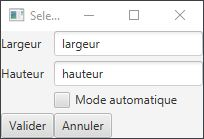
\includegraphics{img/render.javafx/choiceWindow.jpg}
   \end{center}
\end{figure}

Cette fenêtre permet à l'utilisateur de sélectionner la résolution du rendu qu'il souhaite.
Activer le mode automatique maximisera la fenêtre et étendra le rendu sur tout l'écran. Si la résolution sélectionnée est alors inférieur à la résolution de l'écran, la qualité de l'image pourrait s'en trouver altérée.

\subsubsection{La fenêtre d'affichage du rendu}

Une fois que l'utilisateur a entré des paramêtres valides, le rendu s'affichera.

Deux fenêtres s'afficheront alors :

\begin{figure}[h]
   \caption{Fenêtre du rendu}
   \begin{center}
       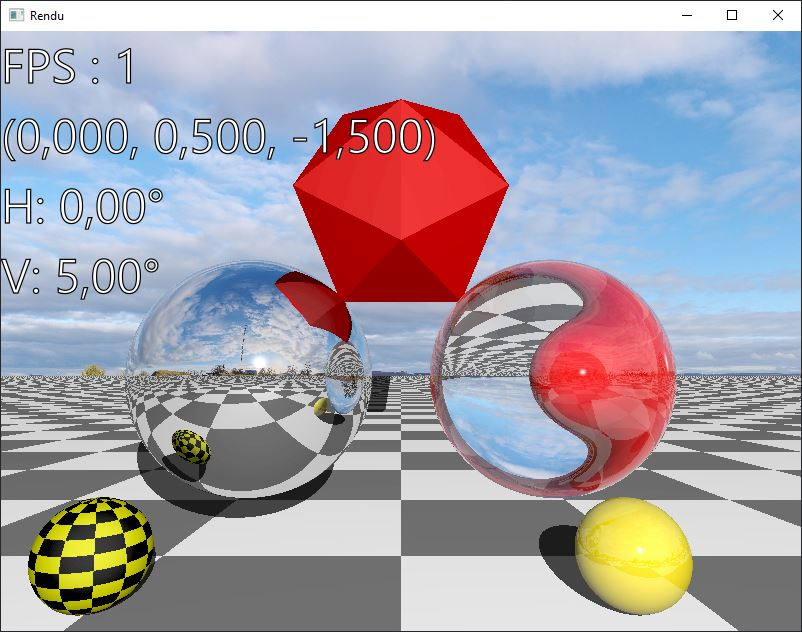
\includegraphics{img/render.javafx/render.jpg}
   \end{center}
\end{figure}

\begin{figure}[h]
   \caption{Fenêtre de la boite à outils}
   \begin{center}
       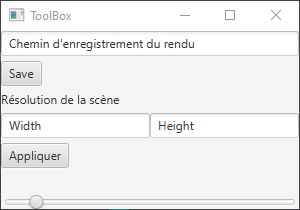
\includegraphics{img/render.javafx/toolbox.jpg}
   \end{center}
\end{figure}

%a déplacer dans readMe.txt

\section{Structuration du projet}
    \subsection{Les packages}
        \subsubsection{Le parser}
        	\subfile{latex/packages/parser_package.tex}
        \subsubsection{Liés au Ray Tracer}
            \subfile{latex/packages/RTpackages.tex}

        \subsection{Le package multithreading}
	  \subfile{latex/packages/multithreading.tex}

	\subsection{Le package geometry}
	    \subfile{latex/packages/geometry.tex}

        \subsection{Le package materials}
            \subfile{latex/packages/materials.tex}

        \subsection{Le package render}
        	Le package render (\figurename\ \ref{diagRender}) contient le code de l'interface graphique, c'est-à-dire celui permettant l'affichage du rendu et des fenêtres.

\begin{description}
    \item [MainApp] contient le main de l'application et lance toutes les fenêtres.
    \item [SetSizeWindow] est la classe responsable de la fenêtre du choix de taille du rendu.
    \item [RenderWindow] est la classe responsable de l'affichage de la fenêtre du rendu.
    \item [Toolbox] est la classe responsable de la fenêtre de changement des réglages du rendu en temps réel.
    \item [CameraTimer] est la classe responsable du déplacement de la caméra lors de l'appui de touches du clavier.
    \item [DoImageTask] est la \textit{Task} contenant les calculs du rendu. Voir la section \ref{UsageTask} pour l'usage des tâches.
\end{description}



\begin{figure}[h]
   \begin{center}
       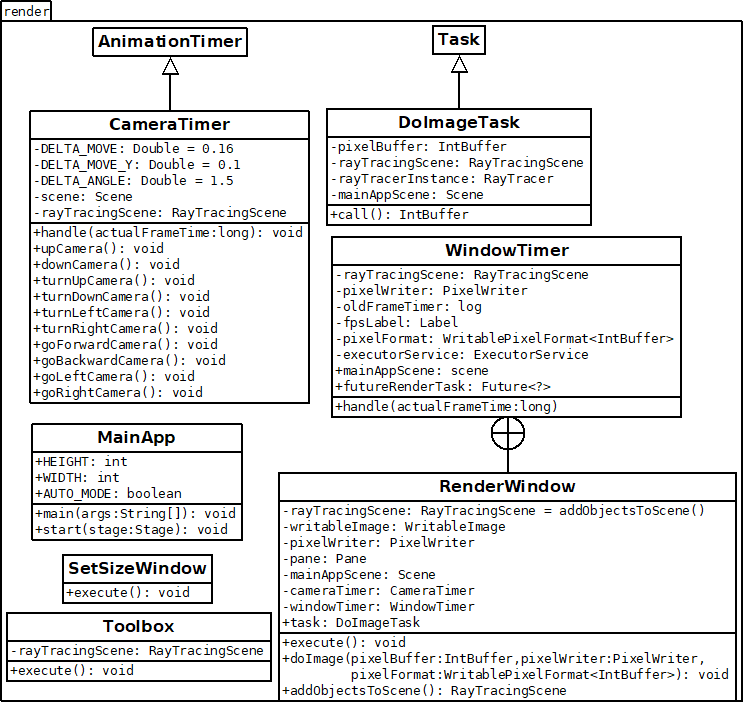
\includegraphics[scale=0.5]{img/render.javafx/diagClassRender.png}
   \end{center}
   \caption{Diagramme du package render \label{diagRender}}
\end{figure}
\FloatBarrier




\section{Détail des parties techniques}
    \subsection{Le Ray Tracer}
        \subsubsection{L'algorithme de base}
            \label{rayTracingBase}

            \subfile{latex/RT/algoBase.tex}

        \subsubsection{L'ombrage de Phong}
            \label{ombragePhong}

            \subfile{latex/RT/ombragePhong.tex}

        \subsubsection{Les réflexions}

            \subfile{latex/RT/reflections.tex}

        \subsubsection{Les réfractions}
            \label{refractions}
            Pour les formules mathématiques de réfractions, nous avons utilisé celle sur le site \href{https://www.scratchapixel.com/lessons/3d-basic-rendering/introduction-to-shading/reflection-refraction-fresnel}{scratchapixel}.
Les matériaux utilisant de la transparence ont un paramètre supplémentaire : l'indice de réfraction. Pour nos tests, nous avons pris celui donné par Wikipedia pour le pyrex(1,474). Nous avions au départ mis un paramètre pour savoir à quel point le materiau était réfractif ou non, mais nous l'avons remplacé par l'équation de fresnel qui calcul la proportion de lumière qui est réfléchie / réfractée. Cette proportion change en fonction de l'angle de pénétration de l'objet, d'où la nécessité de l'emploi de la formule.

\begin{figure}[h]
   \begin{center}
       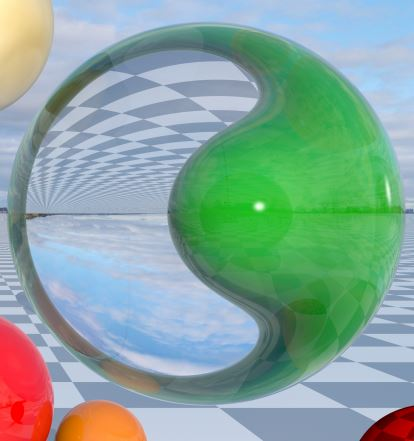
\includegraphics[scale=0.8]{img/rt/refractions.jpg}
   \end{center}
   \caption{Nous pouvons observer une boule verte à travers la boule transparente ainsi que le paysage qui est inversé à cause de la réfraction}
\end{figure}


        \subsubsection{Le damier et le ciel (skybox)}
            \label{checkerboardSkybox}

            \subfile{latex/RT/checkerboardSkybox.tex}

    \subsection{Les formes}
	\subfile{latex/formes/geometryFormes.tex}

    \subsection{Le multithreading}

        \subfile{latex/RT/multithreading.tex}

    \subsection{Les mouvements de caméra}
        \label{mouvementsCamera}

        \subfile{latex/RT/mouvementsCam.tex}

    \subsection{L'interface graphique}

    \subsubsection{Pourquoi JavaFX ?}

Une question que nous nous sommes posée est : Swing ou JavaFX ?

Nous avons choisi d'utiliser JavaFX pour une principale raison. JavaFX est désormais la librairie officielle de Java. Swing n'étant plus maintenu, nous ne voulions pas développer avec une librairie qui commence à être dépréciée.

De plus, le sujet de Bataille Navale (le projet de Complément de POO que nous devons réaliser en parallèle) étant à faire obligatoirement en swing, nous voulions essayer les deux librairies.


\subsubsection{L'interface graphique}

Le développement de l'interface graphique a progressé au rythme du reste du projet, implémentant ce qui a été codé en parallèle. Plusieurs optimisations ont cependant été réalisées pour que l'affichage à l'écran impacte le moins possible les performances générales.

L'optimisation la plus impactant est l'usage d'un IntBuffer et de PixelFormat<IntBuffer>. Ils ont permis d'utiliser la méthode setPixels de PixelWriter, permettant ainsi de définir les pixel de la fenêtre de rendu d'un coup et non pas pixel par pixel comme fait précédememnt.

Un des effets secondaires engendrés par les calculs lourds du rendu est la fenêtre qui n'était plus réactive.
Au départ, nous utilisions CameraTimer et WindowTimer, deux classes héritant de Animation Timer. WindowTimer lançait le rendu et CameraTimer s'occupait de gérer un déplacement de caméra. La méthode handle de AnimationTimer s'exécute à chaque frame, ce qui nous permettait de gérer l'affichage des FPS, la caméra et le rendu à l'aide de la méthode handle et tout était donc synchronisé.

Le problème posé par ce choix était que JavaFX gérait directement les calculs de rendus. La conséquence était une interface graphique réactive à la vitesse du rendu (quelques images par seconde).

\label{UsageTask}

Pour palier à ce problème, nous avons utilisé des classes proposées par le package concurrent de JavaFX. Le problème a été résolu grâce à la classe tasks de ce package, permettant de faire des calculs lourds sans impacter la réactivité de l'interface graphique. Comme javafx et le calcul de rendu n'étaient plus liés il a fallu synchroniser les mouvements de caméra et le calcul de l'image d'après.

\subsubsection{La Toolbox}

La toolbox est un élément essentiel du raytracing. Elle permet à l'utilisateur d'utiliser le logiciel avec simplicité, sans devoir passer par des lignes de commandes ou des scripts d'exécution.
Ensuite, le logiciel de rendu utilise différents procédés qui peuvent fonctionner en parallèle ou les uns au-dessus des autres. La toolbox permet de choisir quels éléments l'utilisateur veux conserver pour pouvoir ainsi mieux comprendre les différentes étapes jusqu'au rendu final.
Pour finir, cette interface permet à l'utilisateur d'avoir un maximum de liberté sur l'utilisation du logiciel, lui permettant ainsi de faire un compromis entre fidélité et rapidité.

\begin{figure}[h]
   \begin{center}
       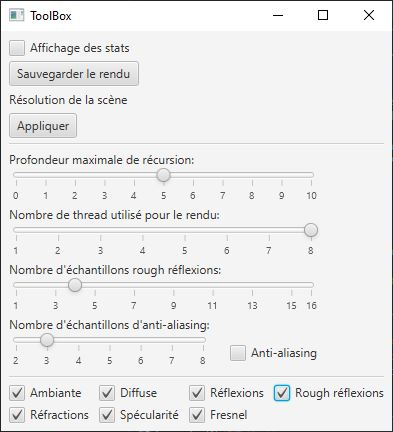
\includegraphics[scale=0.8]{img/rt/toolbox.jpg}
   \end{center}
   \caption{La toolbox et les possibilités qu'elle offre.}
\end{figure}
\FloatBarrier



\subsubsection{Le CSS}

En quelques mots, JavaFX permet de lier le style de ces fenêtres à des fichiers CSS. Nous en avons profité pour aérer les fenêtres de choix de taille et la "toolbox".

\subsubsection{Le mode automatique}

Le mode automatique récupère la taille de l'écran principal, maximise la fenêtre et étire le rendu de manière à ce qu'il soit pixélisé, mais qu'il occupe tout l'écran.

Dans une version plus ancienne, la taille du rendu était également fixée par la taille de la fenêtre. Suite à l'ajout de la réfraction et de l'uvsphère qui sont assez coûteuses en ressource nous avons décidé de supprimer cette fonctionnalité.

\subsubsection{Le compteur de fps}

Le conteur de FPS tire parti des avantages offerts par la classe AnimationTimer et utilise l'horodatage fournit par celle-ci pour calculer la vitesse de rendue.


    \subsection{Le parser}
        \subsubsection{Structure d'un fichier POV}
        	\subfile{latex/parser/struct_pov.tex}
        \subsubsection{Automate à état finit}
           	\subfile{latex/parser/automat.tex}
        \subsubsection{Implémentation du pattern state}
        	\subfile{latex/parser/pattern_state.tex}
        \subsubsection{Implémentation du pattern template méthod}
        	\subfile{latex/parser/pattern_template_method.tex}


    \subsection{Les formes géométriques}




\section{Analyse des résultats}
    \subsection{Mesure des performances}
        \subfile{latex/mesuresPerf.tex}

    \subsection{Comparaison avec povRay}
\section{Idées d'améliorations}
    \subfile{latex/ideesAmelios.tex}
\section{Conclusion}

    Ce projet de rendu 3D par lancée de rayon a été très intéressant à réaliser.
    Grâce à ce travail, nous avons mis en pratique ce que nous avions appris au cours de l'année, mais aussi des éléments que nous n'avions pas étudiés et que nous avons découverts durant le projet.
    De plus, nous avons observé comment les mathématiques et l'informatique peuvent être mises en commun dans un projet, les cours d'algèbres linéaires de L1 nous ayant été d'une grande aide dans plusieurs aspects du logiciel.
    Même s'il restera toujours des perfections à apporter, nous sommes plus que satisfaits du résultat obtenu.




\newpage%Nouvelle page pour les annexes
\subfile{latex/appendices}

\newpage%Nouvelle page pour la bibliographie
\nocite{*}
\bibliographystyle{unsrt}
\bibliography{bibliography/sources}

\end{document}
